\section{Schéma simplifié du cycle de vie d'un projet}
\newImageAnnexe[H]{0.75}{cycle-vie-projet.png}{cycleVieProjet}{Schéma simplifié du cycle de vie d'un projet}

\clearpage
\section{Build continu d'un projet \naq}

{\normalsize Sur ce schéma, on peut constater le retour rapide qui est fait au développeur une fois le code sorti de sa boucle locale (son poste de développeur). Les seules opérations effectuées sont l'installation des dépendances et les tests unitaires, qui prennent quelques secondes à s'exécuter. Cela permet de fournir un retour rapide, via le statut du commit disponible sur Gitlab, qui indique via un badge vert ou rouge le succès ou non des modifications apportées par ce commit.}

\begin{figure}[ht]
	\centering
	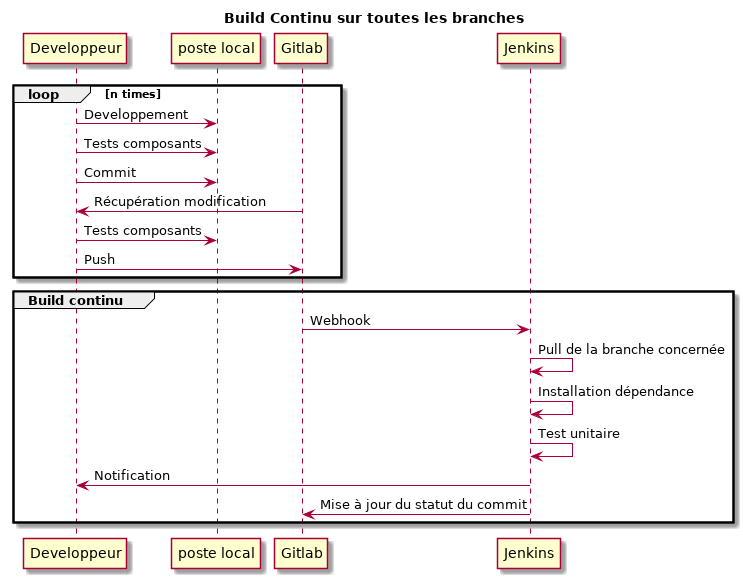
\includegraphics[scale=0.6,angle=-90]{img/build-continu.png}
	\caption{Build continu d'un projet \naq}
	\label{annexe:build-continu}
\end{figure}

\clearpage
\section{Flux de travail du déploiement d'une version d'un site \naq}

\begin{normalsize}
Ce schéma permet de détailler les actions réalisées pour déployer une version d'un site \naq{} en production. Il commence par la demande d'un développeur de lancer un nouveau déploiement. Jenkins, l'outil d'intégration continue, va alors récupérer les dernières sources disponibles sur le \gls{SCM} afin de tester ces dernières. Si les tests sont concluants, Jenkins va alors construire l'application sous forme d'une archive incluant toutes les dépendances nécessaires, en lui attribuant un numéro de version unique incrémenté automatiquement. C'est cette archive qui sera ensuite déployée sur chaque environnement, à commencer par le staging, zone de test interne à l'équipe de développement. Une fois que l'équipe considère que les tests sont valides en staging, l'archive est alors déployée en recette afin d'être mise à disposition du client. Une fois les modifications validées par le client, l'archive est alors déployée en pré-production afin de faire les derniers tests dans un environnement identique à la production. Une fois ces tests passés avec succès, l'application est alors déployée en production et le code est alors rapatrié (\emph{mergé}) de la branche \frquote{develop} sur la branche \frquote{master}. 

On peut constater qu'après chaque déploiement, des \frquote{smoke tests} sont effectués. Ces derniers sont des tests très basiques qui permettent de s'assurer que l'application est stable dans le cas nominal. On va alors tester, dans le cas d'un catalogue d'aide, que les pages d'aides renvoient bien des statuts \gls{HTTP} 200, indiquant que la page répond correctement. Son contenu n'est peut-être pas valide, mais cela indique au moins que le déploiement n'a pas entrainé d'erreurs critiques. 
\end{normalsize}

\newImageAnnexe{0.40}{release.png}{release-naq}{Flux de travail du déploiement d'une version d'un site \naq}

\clearpage
\section{Matrice de développement \devops}

\begin{normalsize}
Source : \url{https://www.infoq.com}

Dans l'image ci-dessous, on peut distinguer une matrice permettant à une entreprise de situer son niveau dans l'adoption d'une démarche \devops. Cette matrice est constituée de 5 niveaux, chacun demandant plus ou moins d'effort pour être atteint et permet de juger 5 points clés, le premier étant la culture de l'entreprise et la façon dont elle est organisée. Cela correspond à la façon l'entreprise va prioriser le travail et organiser les décisions à prendre.

Le second point concerne l'architecture des systèmes que l'entreprise crée. Plus l'entreprise est mature sur ce sujet, plus elle pourra centraliser et versionner chaque changement d'infrastructure, sans avoir à intervenir manuellement sur le projet pour des changements de structure de base de données par exemple. 

Le troisième point concerne la façon dont sont déployées les applications, l'objectif ultime étant de n'avoir aucune intervention humaine sur toute la chaine de déploiement. Le quatrième test concerne la vérification des critères d'acceptations et la qualité des tests mis en place sur le projet. Le dernier point concerne quant à lui la façon dont sont gérés les informations et logs de l'application ainsi que la façon dont ils sont exploités.
\end{normalsize}

\begin{figure}[ht]
	\centering
	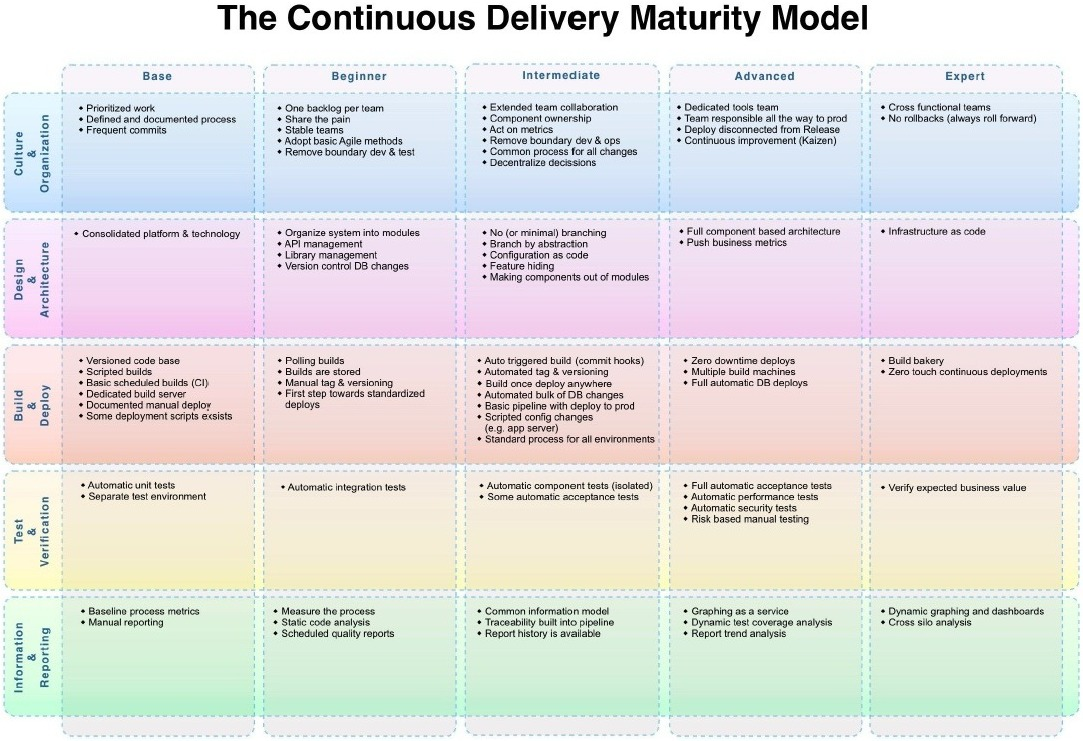
\includegraphics[scale=0.62,angle=-90]{img/devops-matrice.jpg}
	\caption{Matrice de développement \devops}
	\label{annexe:devops-matrice}
\end{figure}

\clearpage
\section{Exemple d'erreurs détectées par PHPStan}

\begin{normalsize}
Dans l'exemple ci-dessous, PHPStan retournera une erreur indiquant que le paramètre requis \frquote{\$type} n'a pas été renseigné, ainsi qu'une erreur indiquant que la méthode privée \frquote{internalBehaviour} ne peut être utilisée en dehors de la classe. 

Il est à noter que cette analyse statique de code peut être et est souvent effectuée au sein de l'\gls{IDE} pour permettre une détection de l'erreur au plus tôt.
\end{normalsize}

%%TC:ignore
\begin{minted}[linenos]{php}
<?php
// index.php

require_once(__DIR__."/vendor/autoload.php");
$a = new \App\File();
$content = $a->loadFile("file.json");
$a->internalBehaviour();

// src/File.php

namespace App;

class File {
  public function loadFile($file, $type) {
    $content = file_get_contents($file);
    if ($type == "json") {
      return json_decode($file);
    }
    return $content;
  }
  
  private function internalBehaviour() {
    echo "this is not public";
  }
}

// ------ ------------------------------------------------------------------- 
// Line   index.php                                                          
// ------ ------------------------------------------------------------------- 
// 6      Method App\File::loadFile() invoked with 1 parameter, 2 required.  
// 7      Call to private method internalBehaviour() of class App\File.      
// ------ ------------------------------------------------------------------- 

\end{minted}
\label{annexe:php-error}
%%TC:endignore
